\section{Diagnóstico de cáncer de mamas}

\subsection{Ejemplos}

Parámetros elegidos:

\begin{itemize}
\item beta = 5
\item mini\_batch\_size = 1
\item lr = 0.005
\item epochs = 1000
\item epsilon = 0.05
\item reg\_param = 0.0
\end{itemize}

\begin{figure}[h]	
	\begin{subfigure}[b]{0.5\textwidth}
		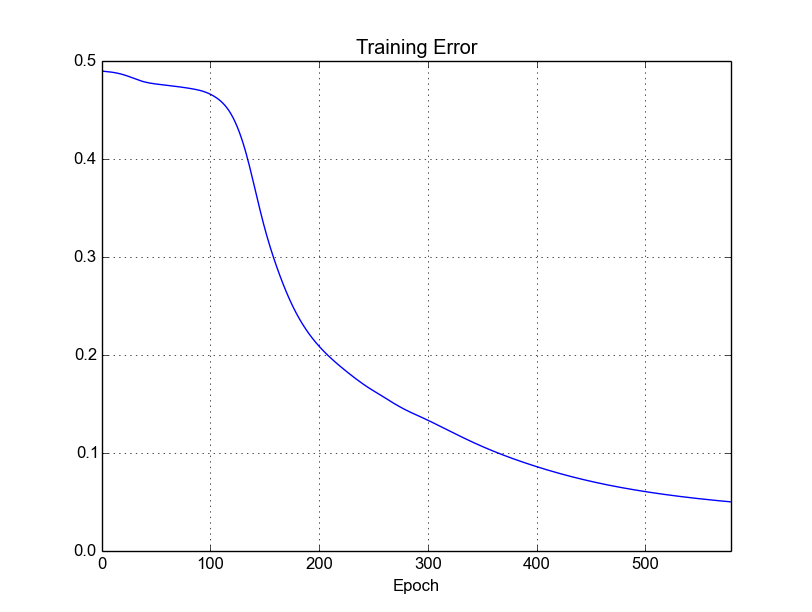
\includegraphics[width=\linewidth]{fig/trainingerror_lr0,005_eps0,05_regparam0,00_beta5_batch1.png}
	\end{subfigure}
	\begin{subfigure}[b]{0.5\textwidth}
		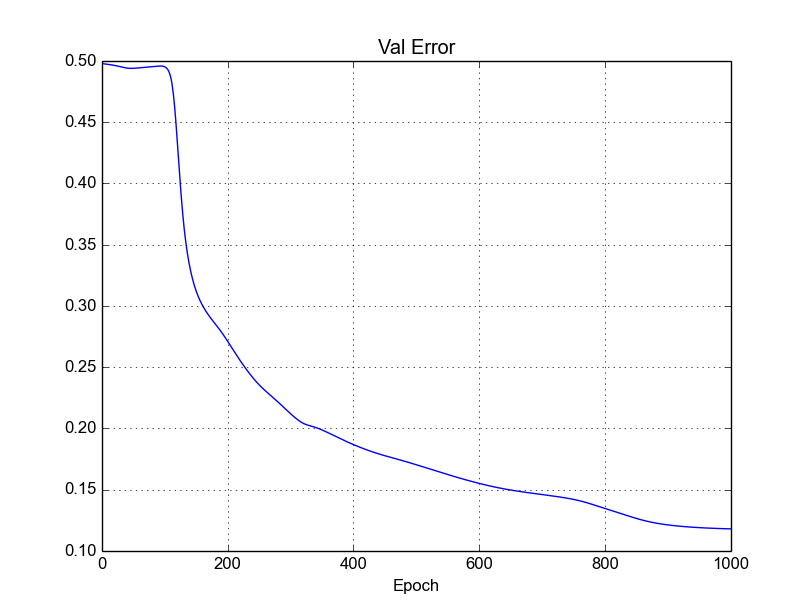
\includegraphics[width=\linewidth]{fig/valerror_lr0,005_eps0,05_regparam0,00_beta5_batch1.png}
	\end{subfigure}

	\caption{error de instancias de entrenamiento vs. error de instancias de validación.}
\end{figure}


\subsection{Código fuente}

\subsubsection*{Carga de datos}

\lstinputlisting[language=Python]{../ej1_data_loader.py}

\subsubsection*{Preprocesamiento de datos}

\lstinputlisting[language=Python]{../preprocessor.py}

\subsubsection*{Modelo}

\lstinputlisting[language=Python]{../layer_model.py}

\subsubsection*{Funciones sigmoideas}

\lstinputlisting[language=Python]{../sigmoid.py}

\subsubsection*{Algoritmos}

\lstinputlisting[language=Python]{../feed_forward_solver.py}

\subsubsection*{Test}

\lstinputlisting[language=Python]{../test2.py}
